\chapter{Modelling}

We used various techniques for the mass modelling of $\omega$ Centauri, so that we could make a good approximation to its dynamic and stellar mass. In order to do this, we decided to use two components (the stellar and dark matter mass) both following the functional form of the Hernquist profile.  

\section{Hernquist Model}

Our modelling is based on the Hernquist profile (Hernquist 1989).  We use this model because it is a well known model that closely approximates the de Vaucouleurs law for elliptical galaxies and has analytical solutions that can be useful for our computational purposes. As introduced in chapter 2, the density profile for this model is

\begin{equation}
\rho(r)=\frac{M}{2\pi}\frac{a}{r}\frac{1}{\left(r+a\right)^{3}}
\end{equation}

Where $a$ and $M$ are the scalength and total mass associated to the profile that, as we will show, can be associated to the dark or baryonic matter. The profile's cumulative mass is

\begin{equation}
M(r)=M\frac{r^{2}}{(r+a)^{2}}
\end{equation}
 
And the surface brightness 
 
 \begin{equation}
 I(R)=\frac{M}{2\pi a^{2}\Gamma\left(1-s^{2}\right)^{2}}\left[\left(2+s^{2}\right)X(s)-3\right]
 \end{equation}
 
where $s=R/a$, $R$ is the projected radius and:

\begin{equation}
X(s)=\frac{1}{\sqrt{1-s^{2}}}\text{sech}^{-1}s \qquad for\qquad0\leq s\leq1
\end{equation}

\begin{equation}
X(s)=\frac{1}{\sqrt{s^{2}-1}}\sec^{-1}s\qquad for\qquad1\leq s<\infty
\end{equation}

For computational simplicity we have written some of the trigonometric functions just like Hernquist did: $\sec^{-1}s = \cos^{-1}(1/s)$ and $\text{sech}^{-1} = \ln[(1+\sqrt{1-s^{2}})/s]$. As mentioned in the theoretical framework chapter, the line of sight velocity dispersion in the more general case with the anisotropy parameter different from 0 we have

\begin{equation}
I(R)\sigma_{p}^{2}(R)=\frac{2}{\Gamma}\int_{R}^{\infty}\left(1-\beta\frac{R^{2}}{r^{2}}\right)\frac{\rho\bar{v_{r}^{2}}rdr}{\sqrt{r^{2}-R^{2}}}
\end{equation}

And the radial velocity dispersion (introduced in chapter 2), in terms of the potential and the density is

\begin{equation}
\bar{v_{r}^{2}}=\sigma_{r}^{2}=\frac{1}{\rho(r)}\int_{r}^{\infty}\rho(r)\frac{d\phi}{dr}dr
\end{equation}

Where 

\begin{equation}
\frac{d\phi}{dr}=\frac{GM(r)}{r^{2}}
\end{equation}

So the projected velocity dispersion becomes:

\begin{equation}
\sigma_{p}^{2}(R)=\frac{2G}{I(R)\Gamma}\int_{R}^{\infty}\left(1-\beta\frac{R^{2}}{r^{2}}\right)\left(\int_{r}^{\infty}\frac{\rho(r)M(r)}{r^{2}}dr\right)\frac{rdr}{\sqrt{r^{2}-R^{2}}}
\end{equation}

We do various experiments for our modelling, the simplest of all models is the one where we assume that the cluster has just one mass component, in this case there only will be one mass contribution and only one scalength (the stellar scalength) so the solution of the last equation would be:

\begin{equation}
\sigma_{p}^{2}(R)=\frac{GM^{2}a}{I(R)\Gamma\pi}\int_{R}^{\infty}\alpha(r)\left(\frac{\log{\left(\frac{a+r}{r}\right)}}{a^{5}}-\frac{25a^{3}+52a^{2}r+42ar^{2}+12r^{3}}{12a^{4}\left(a+r\right)^{4}}\right)dr
\end{equation}

Where $a$ is the scalength and where, in order to shorten the equation we take $\alpha(r)$ as 

\begin{equation}
\alpha(r)=\left(1-\beta\frac{R^{2}}{r^{2}}\right)\frac{r}{\sqrt{r^{2}-R^{2}}}
\end{equation}

Now, as we want to focus on the dark matter content of the cluster, we assume that the mass of the cluster is the sum of the mass of stars and the mass of non-baryonic matter so that their contributions to the density and mass profiles become:

\begin{equation}
\rho(r)=\rho_{s}(r)+\rho_{dm}(r)\qquad and \qquad M(r)=M_{s}(r)+M_{dm}(r)
\end{equation} 

In this case, the projected velocity dispersion takes a much more complicated form as follows:

\begin{equation}
\begin{aligned}	
\sigma_{p}^{2}(R) &= \frac{G}{I(R)\Gamma\pi}\int_{R}^{\infty}\alpha(r)\Biggl[\underbrace{\int_{r}^{\infty}\frac{M_{s}^{2}a_{s}dr}{r\left(r+a_{s}\right)^{5}}}_{\mathbf{A}(r)}+\underbrace{\int_{r}^{\infty}\frac{M_{s}M_{dm}a_{s}dr}{r\left(r+a_{s}\right)^{3}\left(r+a_{dm}\right)^{2}}}_{\mathbf{B}(r)}\right\\     &+ \underbrace{\int_{r}^{\infty}\frac{M_{dm}M_{s}a_{dm}dr}{r\left(r+a_{dm}\right)^{3}\left(r+a_{s}\right)^{2}}}_{\mathbf{C}(r)}+\underbrace{\int_{r}^{\infty}\frac{M_{dm}^{2}a_{dm}dr}{r\left(r+a_{dm}\right)^{5}}}_{\mathbf{D}(r)}\Biggr] dr
\end{aligned}
\end{equation}

The functional form of the density involves the use of a stellar scalength ($a_{s}$), a dark matter scalength ($a_{dm}$), a stellar mass ($M_{s}$) and a dark matter mass ($M_{dm}$). Now, the integrals $\mathbf{A}(r),\mathbf{B}(r),\mathbf{C}(r)$ and $\mathbf{D}(r)$ have the following analytical solutions:

\begin{equation}
\textbf{A}(r)=a_{s}\left(-\frac{25a_{s}^{3}+52a_{s}^{2}r+42a_{s}r^{2}+12r^{3}}{12a_{s}^{4}\left(a_{s}+r\right)^{4}}+\frac{\log{\left[\frac{a_{s}+r}{r}\right]}}{a_{s}^{5}}\right)
\end{equation}

\begin{equation}
\textbf{D}(r)=a_{dm}\left(-\frac{25a_{dm}^{3}+52a_{dm}^{2}r+42a_{dm}r^{2}+12r^{3}}{12a_{dm}^{4}\left(a_{dm}+r\right)^{4}}+\frac{\log{\left[\frac{a_{dm}+r}{r}\right]}}{a_{dm}^{5}}\right)
\end{equation}

\begin{equation}
\textbf{B}(r)=\frac{\left(M_{s}M_{dm}\right)\left(\mathbf{b_{2}}+\mathbf{b_{3}}+a_{s}\left(-\left(a_{s}-a_{dm}\right)a_{dm}\mathbf{b_{4}}+\mathbf{b_{5}}\right)\right)}{\mathbf{b_{1}}}
\end{equation}

\begin{equation}
With \left\lbrace
\begin{array}{lllll}
\mathbf{b_{1}}=2a_{s}^{2}(a_{s}-a_{dm})^{4}a_{dm}^{2}(a_{s}+r)^{2}(a_{dm}+r)\\
\mathbf{b_{2}}=-2\left(a_{s}-a_{dm}\right)^{4}\left(a_{s}+r\right)^{2}\left(a_{dm}+r\right)\log{r}\\
\mathbf{b_{3}}=2a_{dm}^{2}\left(6a_{s}^{2}-4a_{s}a_{dm}+a_{dm}^{2}\right)
\left(a_{s}+r\right)^{2}\left(a_{dm}+r\right)\log{[a_{s}+r]}\\
\begin{aligned}	
\mathbf{b_{4}} &= 2a_{s}^{4}+4a_{s}^{3}r-2a_{dm}r(a_{dm}+r)+3a_{s}a_{dm}\left(-a_{dm}^{2}+a_{dm}r+2r^{2}\right)\\      &+a_{s}^{2}\left(7a_{dm}^{2}+7a_{dm}r+2r^{2}\right)
\end{aligned}\\
\mathbf{b_{5}}=2a_{s}^{2}\left(a_{s}-4a_{dm}\right)\left(a_{s}+r\right)^{2}\left(a_{dm}+r\right)\log{[a_{dm}+r]}
\end{array}
\right.
\end{equation} 

And

\begin{equation}
\textbf{C}(r)=\frac{\left(M_{dm}M_{s}\right)\left(\mathbf{c_{2}}+\mathbf{c_{3}}+a_{dm}\left(-\left(a_{dm}-a_{s}\right)a_{s}\mathbf{c_{4}}+\mathbf{c_{5}}\right)\right)}{\mathbf{c_{1}}}
\end{equation}

\begin{equation}
With \left\lbrace
\begin{array}{lllll}
\mathbf{c_{1}}=2a_{dm}^{2}(a_{dm}-a_{s})^{4}a_{s}^{2}(a_{dm}+r)^{2}(a_{s}+r)\\
\mathbf{c_{2}}=-2\left(a_{dm}-a_{s}\right)^{4}\left(a_{dm}+r\right)^{2}\left(a_{s}+r\right)\log{r}\\
\mathbf{c_{3}}=2a_{s}^{2}\left(6a_{dm}^{2}-4a_{dm}a_{s}+a_{s}^{2}\right)\left(a_{dm}+r\right)^{2}
\left(a_{s}+r\right)\log{[a_{dm}+r]}\\
\begin{aligned}	
\mathbf{c_{4}} &= 2a_{dm}^{4}+4a_{dm}^{3}r-2a_{s}r(a_{s}+r)+3a_{dm}a_{s}\left(-a_{s}^{2}+a_{s}r+2r^{2}\right)\\      &+a_{dm}^{2}\left(7a_{s}^{2}+7a_{s}r+2r^{2}\right)
\end{aligned}\\
\mathbf{c_{5}} =2a_{dm}^{2}\left(a_{dm}-4a_{s}\right)\left(a_{dm}+r\right)^{2}\left(a_{s}+r\right)\log{[a_{s}+r]}
\end{array}
\right.
\end{equation} 

As we mentioned in the last chapter, we used many databases for projected radial velocities in order to properly do our fit and modelling. The radial velocities as a function of the projected radius is shown in figure 4.1

\begin{figure}[H]
\centering
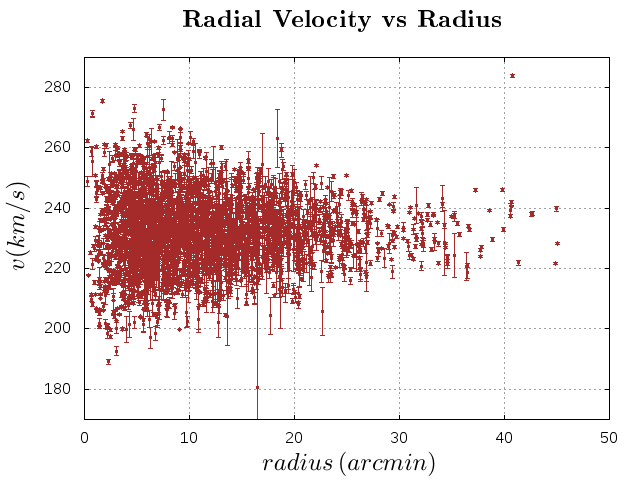
\includegraphics[width=11cm]{images/vel_vs_rad.png}
\caption[Radial velocity database]{Radial velocities vs projected radius in arcmin. The data is taken from all the databases that gave us a good level of confidence, note that all the data have their respective error.}
\end{figure}

Because we need to calculate the projected velocity dispersion profile, we need to cut in radial bins as shown in figure 4.2. 

\begin{figure}[H]
\centering
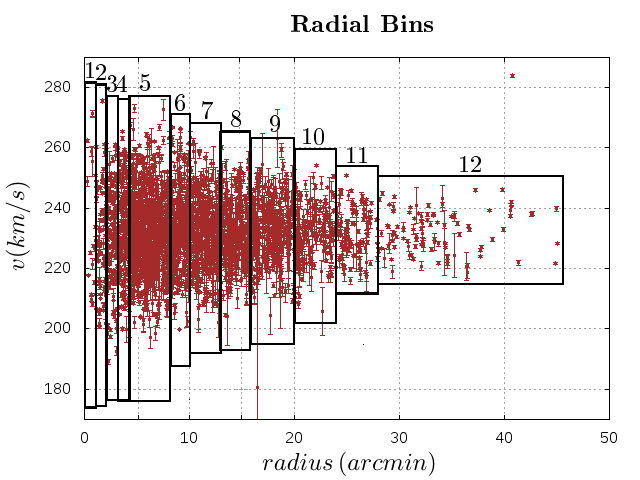
\includegraphics[width=11cm]{images/vel_vs_rad_bins.png}
\caption[Radial bins used to calculate velocity dispersions]{Radial bins that we use to calculate the radial projected velocity dispersion in the cluster using equation 4.20}
\end{figure}

The velocity dispersion is estimated as the standard deviation of the velocity in each radial bin because we want to see how much the velocity data deviates from the median, and it is calculated with the formula

\begin{equation}
\sigma = \sqrt{\frac{\sum_{i=1}^{n}\left(v_{i}-v\right)^{2}}{N}}
\end{equation}

To see if the estimation is well made, we plot histograms for each bin to see if the velocities follow a Gaussian behaviour, and where the number of bars in each histogram is given by the square root of the number of velocities in each bin. For some of the radial bins of our profile, the histograms are shown in figure 4.3

\begin{figure}[H]
\centering
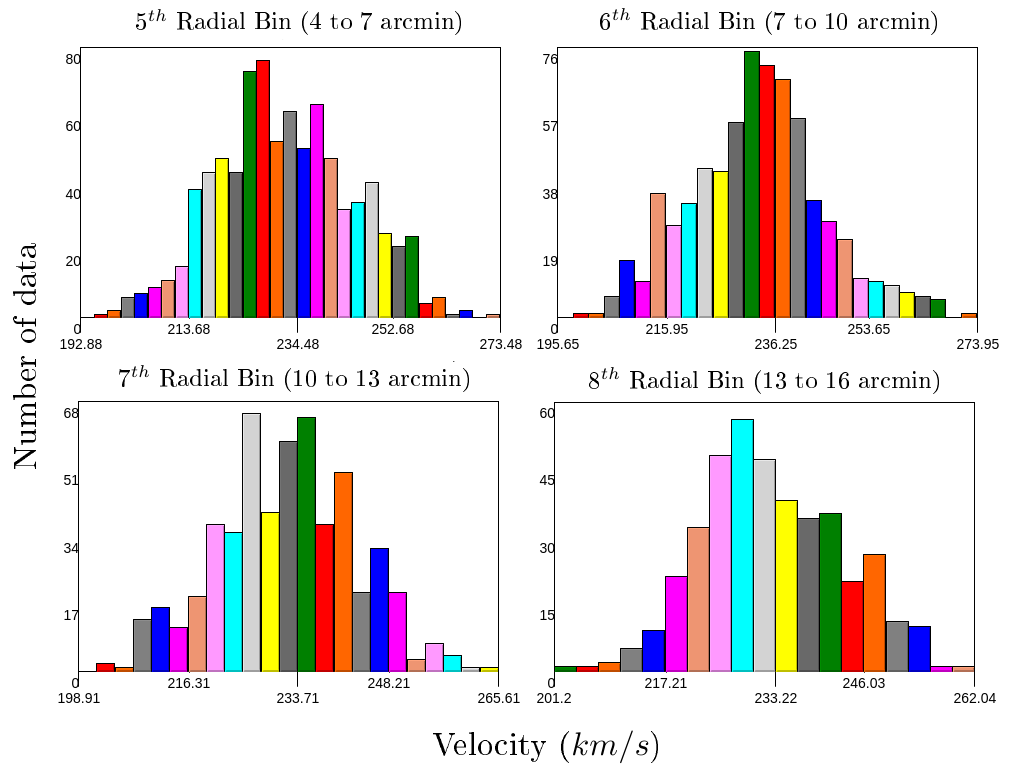
\includegraphics[width=15cm]{images/bines.png}
\caption[Histograms for some of the radial bins in our profile]{The histograms for the $5^{th}$, $6^{th}$, $7^{th}$ and $8^{th}$ radial bins. Note that the frequency of repetition of the velocities displayed in bars follows a Gaussian behaviour which suggests that the method used to calculate the velocity dispersion in accurate enough for the modelling.}
\end{figure}

In order to do a proper modelling and fitting we need to take into account the error associated with $\sigma_{p}$. Because all the databases provided the associated error to the measurements of the radial velocities, we made the proper calculation of the error of the velocity dispersion using the general error propagation formula

\begin{equation}
\sigma(v\pm\Delta v)\approx \sigma(v)\pm \underbrace{\frac{\partial \sigma}{\partial v}\Delta v}_{\Delta \sigma}
\end{equation}

So the error of the projected velocity dispersion is estimated as

\begin{equation}
\Delta \sigma = \frac{1}{\sqrt{N}}\left(\sum_{i=1}^{n}\left(v_{i}-v\right)^{2}\right)^{-1/2}\sum_{i=1}^{n}\left(v_{i}-v\right)\Delta v
\end{equation}

With the radial projected velocity dispersion (and its error) we can start with the fitting to find the optimized parameters in our various experiments. Because the functions that we wanted to fit did not have an analytic solution, we decided use a $\chi^{2}$ method instead. 

This approximation method allows to fit curves to the observational data so that the parameters would be optimized, that is, the combination of parameters would allow the curve to fit well the observational data. Our programs were set so that the $\chi^{2}$ was calculated for every combination of the parameters (every entry of the parameters matrix) but it will only save the values of the parameters that make the smallest $\chi^{2}$. If we call $\sigma_{M}(r_{i})$ the value of our modelling for the radial bin $i$ and if $\sigma_{i}$ is the observational value of the projected velocity dispersion in the same bin, we show that our calculation of this approximation method is given by 

\begin{equation}
\chi^{2}=\sum_{i=1}^{n}\frac{1}{N_{i}}{\left(\sigma_{M}\left(r_{i}\right)-\sigma_{i}\right)}^{2}
\end{equation}

Where $N_{i}$ is the number of velocities used to calculate the velocity dispersion in bin $i$ (this was included to give more weight to the radial bins that were calculated with a higher number of data), and $n$ is the number of radial bins.

\section{Setting constraints}

\subsection{Stellar Population Synthesis with Starlight}

The stellar mass content of Globular Clusters and Galaxies can be studied through the determination of the stellar populations inside those systems because we have clear knowledge about how their photometric properties relate to their mass. If we have information about the relative abundance of the stellar populations inside the stellar system, then we can infer the total mass of the cluster by summing up all of these contributions. 

The determination of the stellar populations can be done using STARLIGHT, which is a Fortran-based program that fits an observed integrated spectrum (Omega Centauri in our case) with a model spectrum which is the sum of $N_{*}$ spectral components from a pre-defined and pre-processed set of base spectra. The program does as many iterations as the user decides to sum up the different template spectra until a good fitting of the spectral lines has been made to the observed spectrum. 

The output of the program after the execution contains the created spectrum (wavelength and intensity) and the approximate percentage of each of the stellar populations inside the stellar system that we use for the determination of the total mass of the cluster.

First, one must prepare the observed spectrum before running STARLIGHT, the spectrum has to be wavelength and flux calibrated, taking into account the bad-pixel removal. Very importantly in the context of mass analysis, the spectrum has to be extinction corrected so that the units of flux relate properly to the units of the templates in STARLIGHT.     

The extinction correction for our observed spectrum is given by

\begin{equation}
f_{obs}(\lambda)=f_{int}(\lambda)10^{-0.4A_{\lambda}}
\end{equation}

Where $A_{\lambda}=0.213$ in the I filter around $8000 \textrm{\AA}$, around the wavelength range of our spectrum. 

In our case, we have to multiply by a factor of 1.216746 the intensity of the spectrum to correct of extinction. After we apply the extinction correction to the spectrum and create an ASCII table with the wavelength, intensity and error columns, it is now ready to be processed with STARLIGHT as we can see in the figure 4.9.

\begin{figure}[H]
\centering
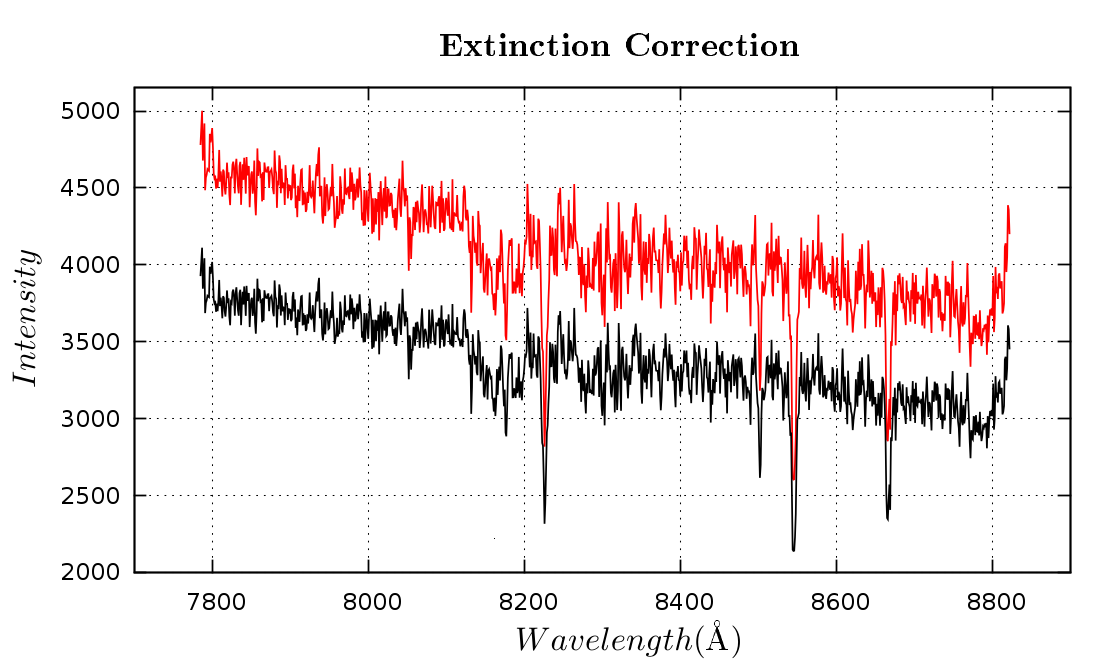
\includegraphics[width=10cm]{images/extinction.png}
\caption[Extinction Correction]{This figure shows an integrated spectrum of the central region of Omega Centauri before and after the extinction correction is applied. The black line has the original flux values and the black line has the corrected flux, that is, the flux that would be observed if there wasn't any interstellar medium that obscures the light coming from the object.}
\end{figure}

Before running STARLIGHT one must assure that the wavelength range is correctly specified in the configuration file that also includes the database of the template spectra and the bad data organized in a mask file. When all of these are ready it is straightforward to run STARLIGHT with the following command (in a linux-based computer):

\begin{center}
./StarlightChains\_v04.exe $<$ Omega\_cen.in
\end{center}

The synthetic spectrum and the original one are shown in figure 4.10.

\begin{figure}[H]
\centering
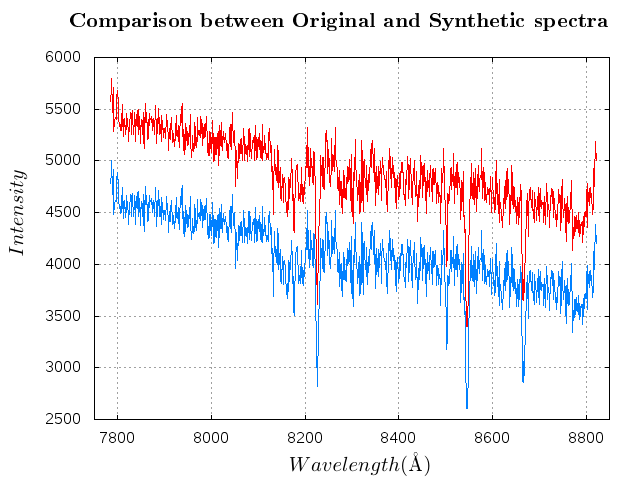
\includegraphics[width=10cm]{images/comparison.png}
\caption[Synthetic spectrum of STARLIGHT]{Synthetic spectrum of Starlight in red, shifted in the y axis for doing the comparison with the original spectrum of Omega Centauri in blue. Note how similar the spectra are, meaining that the results given by Starlight were very accurate}
\end{figure}
 
Now, besides the synthetic spectrum, the output file contains some useful results that one can use to estimate the mass of the stellar system. In our case, the relevant parameter that STARLIGHT gives is the ``stellar mass parameter":

\begin{equation}
M_{cor\_tot} = 3.29446 \times 10^{7} M_{\odot}/cm^{2}
\end{equation}

And using the formula for the total mass in units of solar masses:

\begin{equation}
M_{s}(M_{\odot})=M_{cor\_tot}\times10^{-17}\times4\pi d^{2}\times\left(3.826\times10^{33}\right)^{-1}
\end{equation}

Where $d$ is the luminosity distance in cm. This equation yields a stellar mass of $M_{\star}=243.462M_{\odot}$

This mass is the stellar mass contained in the detection area (that in our set up configuration in OPD ends up to be $A_{D}=0.36\,pc^{2}$) of the integrated spectrum that we analysed with STARLIGHT so if we want to calculate the whole stellar mass of the system we must extrapolate this result to its whole effective area, noting that this will increase the error of the calculation.

If we take the cluster's tidal radius of 40' and it's distance to the sun of $4808.39\,pc$ using a distance modulus of 13.41, then the total effective area (where the stellar mass could be calculated using stellar population synthesis) is $A_{OC}=9833.8\,pc^{2}$. 

Finally, the total stellar mass of the Cluster using this technique can be calculation using:

\begin{equation}
M_{s T} = N \times M_{\star}
\end{equation}

Where N is the number of detection areas within the total effective area of Omega Centauri ($A_{OC}/A_{D}$) of about 31844.8. So that our calculation of the stellar mass is finally:

\begin{equation}
M_{s T} = 6.61 \times 10^{6}M_{\odot}
\end{equation}
 
This result is actually larger than some values  of the dynamical mass found in the literature and it should in principle, be smaller or at least equal to the dynamical mass, this discrepancy in our first approach to the mass determination is probably due to errors given by the extrapolation of the results of the detection area to the whole area of the cluster, because our detection area was very small ($\sim 0.2 \, arcmin^{2}$) compared to the cluster's size of more than $6,000 \, arcmin^{2}$. Still, the stellar population technique is consistent with the order of magnitude of the cluster's mass previously reported. 


This first set of experiments consisted of the variation of every parameter of our modelling, that is, dark matter mass $M_{dm}$, stellar mass $M_{s}$, dark matter scalength $a_{dm}$, stellar scalength $a_{s}$, mass-to-light ratio $\Gamma$ and parameter of anisotropy $\beta$.

Because some authors (Jalali et al. 2012) state that there might be a medium-mass black hole at the center of $\omega$ Centauri, we decided to conduct two different fittings, one with the central region of the cluster (12 radial bins) and other without the central region of the cluster (10 radial bins), and in each group of experiments we made four basic assumptions to take into account all the possibilities of our modelling:

\textbf{\textit{i)}} In this one, we don't use the crossed terms in equation 4.13, because we wanted to see how relevant they were in the modelling, we call this ``\textbf{\textit{No crossed terms}}". 

\textbf{\textit{ii)}} We assume a constant stellar scalength, we call this ``\textbf{\textit{Fix $a_{s}$}}". Because we wanted to be as accurate as possible in our modelling we found a way to calculate the stellar scalength and use is as a constraint to our modelling. We found the value of $a_{s}$ by fitting the effective radius in a de Vaucouleurs profile on the surface brightness of Eva Noyola's observational data (Noyola et al. 2013) shown in figure 4.4

\begin{figure}[H]
\centering
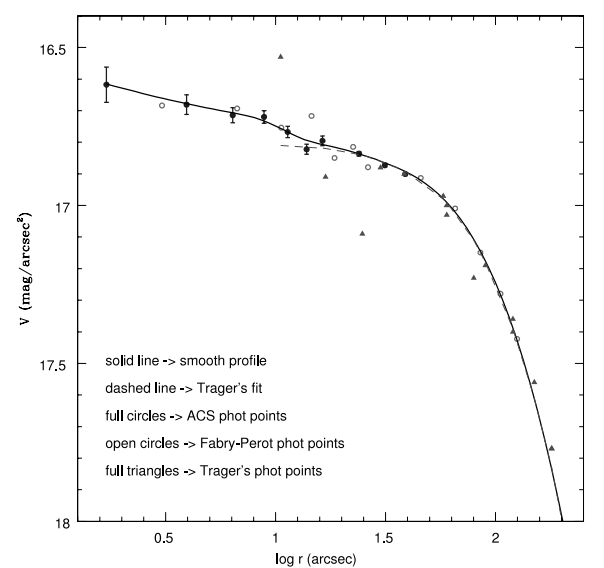
\includegraphics[width=11cm]{images/noyola.png}
\caption[Surface brightness profile of Omega Centauri]{Surface brightness profile for $\omega$ Centauri. The circles show
Noyola's measured photometric points. The triangles show photometric points obtained from ground based images by Trager et al. The dashed line is Trager’s Chebychev fit. The solid line is Noyola's smooth fit that we don't use for our fitting of the scalength. Figure taken from Noyola et al. 2013}
\end{figure}

Our fitting gives us an effective radius of $R_{e}=4.048$ and using the relation $R_{e}\approx1.8153a$ (Hernquist 1989), we find a stellar scalength of $a_{s}=2.23$ that we use for our set of experiments.

\textbf{\textit{iii)}} We don't assume any of our parameters to be constant, that is, we vary $a_{s}$, $a_{dm}$, $\gamma$, $\beta$, $M_{dm}$ and $M_{s}$ in the parameter matrix, we call this ``\textbf{\textit{Full}}". 

\textbf{\textit{iv)}} We assume the cluster doesn't have any dark matter so the solution of the equation 4.9 is much simpler and it's given by 4.10, we call this ``\textbf{\textit{No Dark matter}}".

Now we describe one by one the experiments we made to model the mass distribution of the globular cluster using the $\chi^{2}$ minimization technique.

%\newpage

\section{Results}

\subsection{Full Modelling including the inner region of the cluster}

In this set of experiments we do the variation of all the parameters and we use the whole sample of 12 velocity dispersions to be fitted. The results are summarized in figure 4.5 and table 4.1.

\begin{figure}[H]
\centering
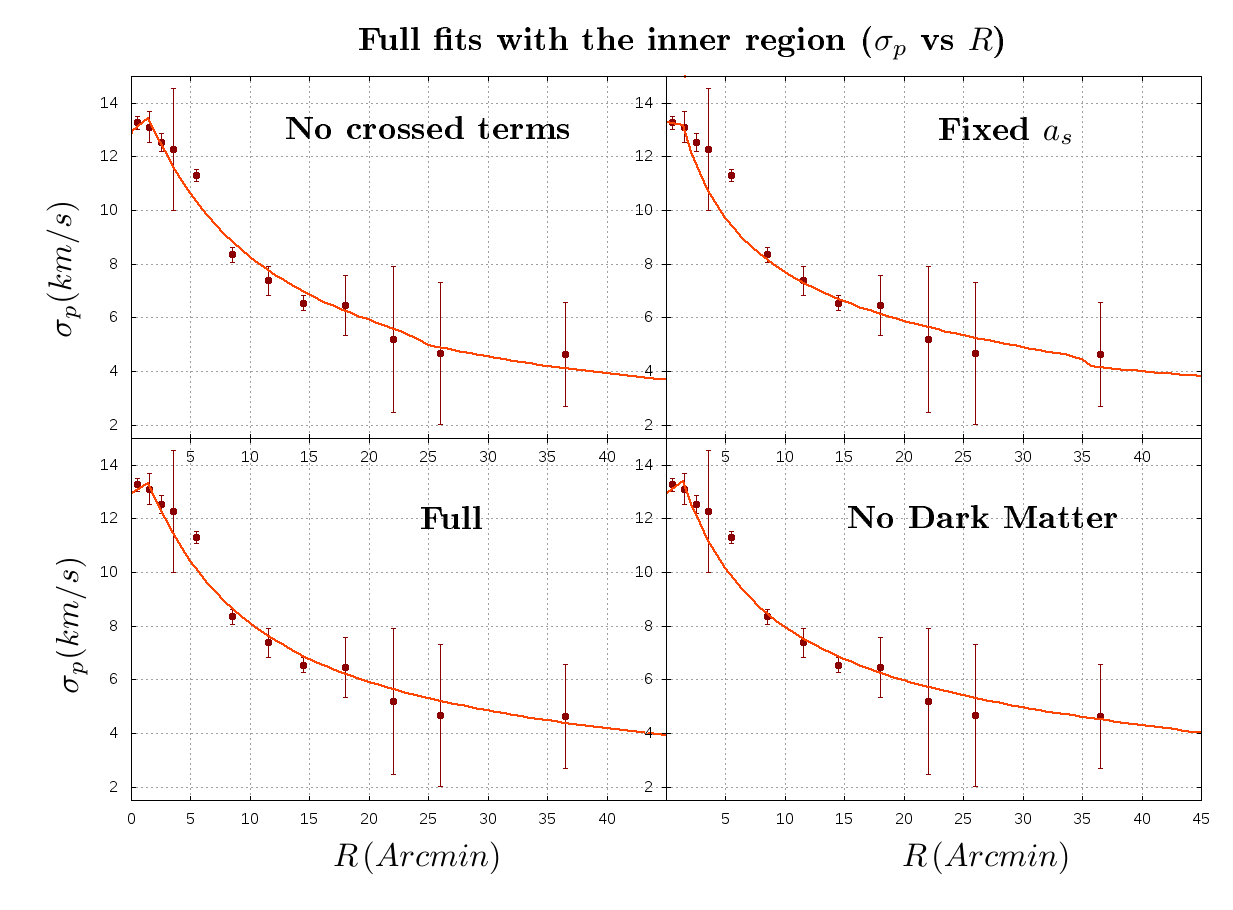
\includegraphics[width=15cm]{images/all_params_refinado_12.png}
\caption[Best fit of the full model for 12 radial bins]{Best fit to the observational data of the four experiments for our full model with the 12 radial bins.}
\end{figure}

\begin{table}[H]
\begin{center}
\begin{tabular}{| c | c | c | c | c | c | c| }
    \hline
    \textbf{Experiment} & $\mathbf{\beta}$ & $\mathbf{a_{dm}} (pc)$ & $\mathbf{a_{s}} (pc)$ & $\mathbf{M_{dm}}$ ($M_{\odot}$) & $\mathbf{M_{s}}$ ($M_{\odot}$) & $\mathbf{\Gamma}$\\ \hline
	No Crossed terms & $0.62$ &	$15.8$ &	$29.0$ &	$5.6 \times 10^{5}$ &	$8.0 \times 10^{4}$ &	$2.2$\\ \hline
	Fix $a_s$ &	$0.0001$ &	$9.0$ &	$2.23$ &	$1.12 \times 10^{5}$ &	$1.06 \times 10 ^{6}$ &	$1.5$\\ \hline
	Full &	$0.46$ &	$15.2$ &	$52.6$ &	$9 \times 10^{5}$ &	$9 \times 10^{5}$ &	$0.38$\\ \hline
	No Dark Matter &	$0.26$ & $\thicksim$	& $ a = 3.64$  & $\thicksim$ & $  M = 1.98 \times 10^{6}$ & 	$1.24$\\
    \hline
  \end{tabular} 
\caption[Optimized parameters for our full model with the 12 radial bins.]{The optimized parameters for each of the experiments for our full model with the 12 radial bins.}
\end{center}
\end{table}

%\newpage

\subsection{Full Modelling for the outer region of the cluster}

In this set of experiments we do the variation of all the parameters and we use the 10 of the 12 points of the velocity dispersions because we want to avoid the problems in the center of the cluster and search for a smoother behaviour in the fitting of our model. The results are summarized in figure 4.6 and table 4.2.

\begin{figure}[H]
\centering
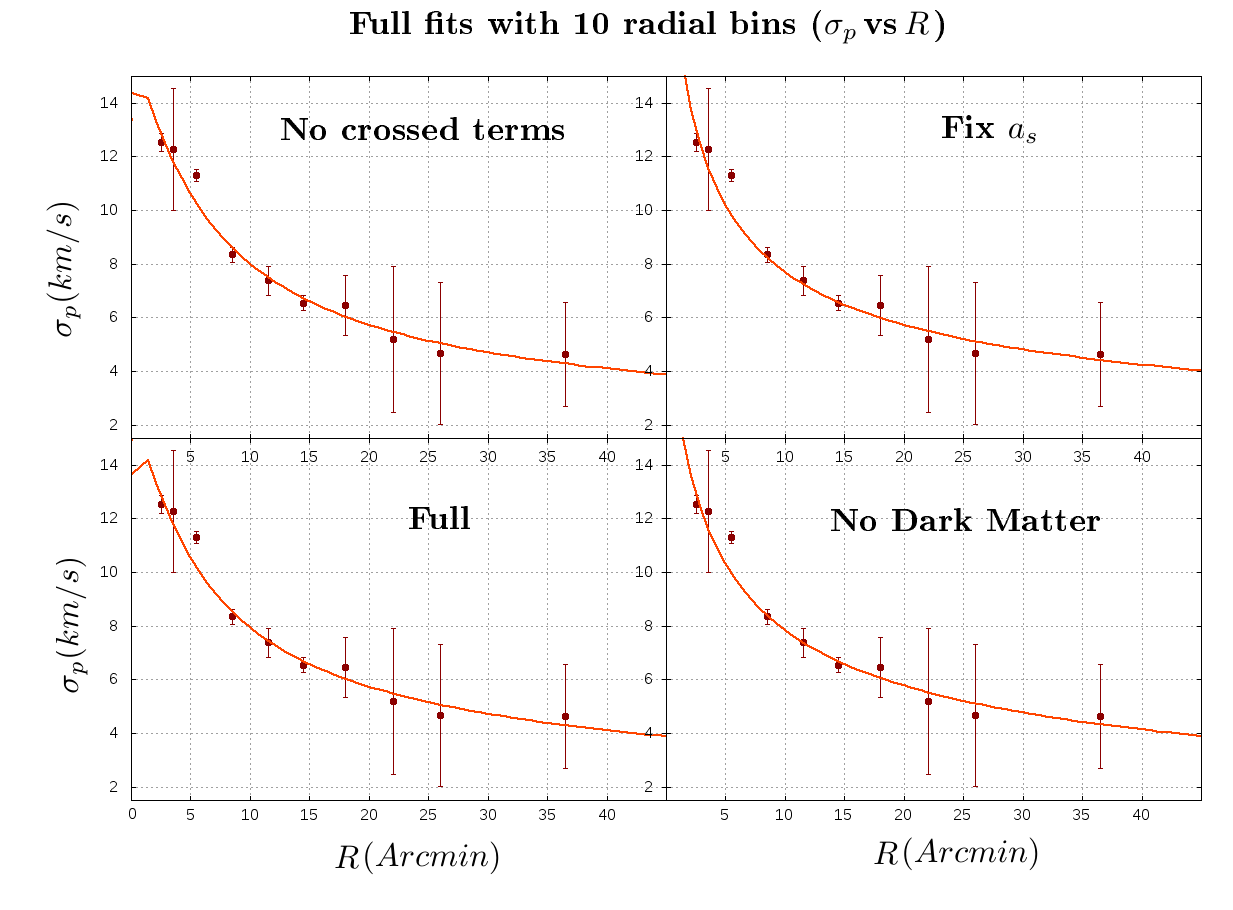
\includegraphics[width=15cm]{images/all_params_refinado_10.png}
\caption[Best fit of the full model for 10 radial bins]{Best fit to the observational data of the four experiments for our full model with the 10 outer radial bins.}
\end{figure}

\begin{table}[H]
\begin{center}
\begin{tabular}{| c| c| c| c| c| c| c|}
    \hline
    \textbf{Experiment} & $\mathbf{\beta}$ & $\mathbf{a_{dm}} (pc)$ & $\mathbf{a_{s}} (pc)$ & $\mathbf{M_{dm}}$ ($M_{\odot}$) & $\mathbf{M_{s}}$ ($M_{\odot}$) & $\mathbf{\Gamma}$\\ \hline
	No Crossed terms & $0.6$ &	$16$ &	$52.8$ &	$2.1 \times 10^{6}$ &	$2.72 \times 10^{6}$ &	$2.3$\\ \hline
	Fix $a_s$ &	$0.79$ &	$57.9$ &	$2.23$ &	$8 \times 10^{5}$ &	$3.43 \times 10 ^{6}$ &	$2.1$\\ \hline
	Full &	$0.04$ &	$11.8$ &	$57.8$ &	$6 \times 10^{5}$ &	$9 \times 10^{5}$ &	$2.1$\\ \hline
	No Dark Matter &	$0.78$ &	$\thicksim$ & $ a = 2.96$ &	$\thicksim$ & $  M = 3 \times 10^{6}$ & 	$1.94$\\
    \hline
  \end{tabular} 
\caption[Optimized parameters for our full model with the 10 outer radial bins.]{The optimized parameters for each of the experiments for our full model with the 10 outer radial bins.}
\end{center}
  
\end{table}

%\subsection{Fix mass-to-light ratio}

In the following set of experiments, the mass-to-light ratio we used was $\Gamma = 2.5$ (Van de Ven et al. 2005) and the results were the following: 

\subsection{Fix mass-to-light ratio including the inner region of the cluster}


We vary all the parameters except for the mass to light ratio $\Gamma$ that, as we just showed, has a value of $2.5$ and we use 12 points to fit the model. The results are summarized in figure 4.7 and table 4.3.

\begin{figure}[H]
\centering
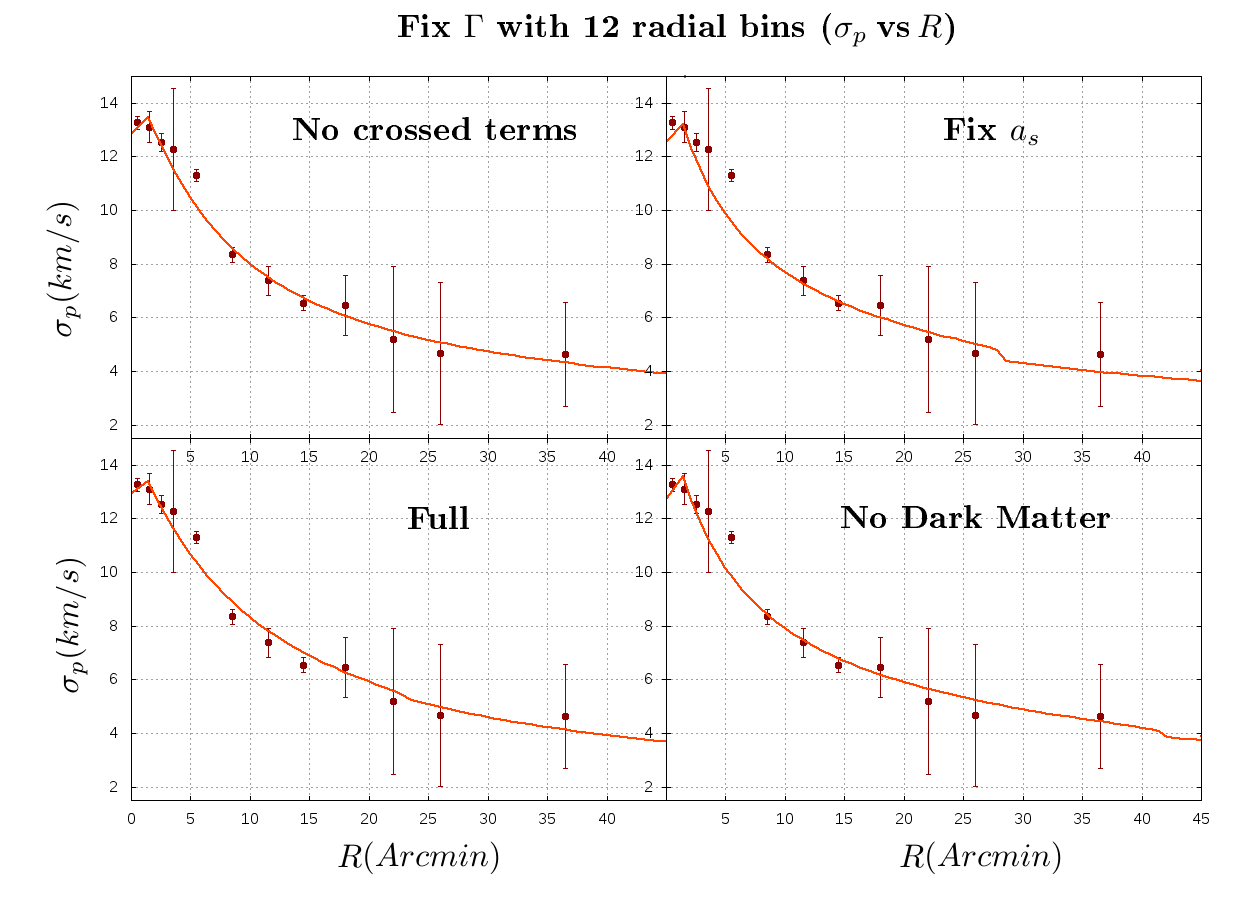
\includegraphics[width=15cm]{images/fix_gamma_refinado_12.png}
\caption[Best fit of our model with a fix mass-to-light ratio for the 12 radial bins]{Best fit to the observational data of the four experiments for our model with a fix mass-to-light ratio with the 12 radial bins.}
\end{figure}

\begin{table}[H]
\begin{center}
\begin{tabular}{| c| c| c| c| c| c| c|}
    \hline
    \textbf{Experiment} & $\mathbf{\beta}$ & $\mathbf{a_{dm}} (pc)$ & $\mathbf{a_{s}} (pc)$ & $\mathbf{M_{dm}}$ ($M_{\odot}$) & $\mathbf{M_{s}}$ ($M_{\odot}$) & $\mathbf{\Gamma}$\\ \hline
	No Crossed terms & $0.35$ &	$16.4$ &	$55.62$ &	$1.62 \times 10^{6}$ &	$2.1 \times 10^{6}$ &	$2.5$\\ \hline
	Fix $a_s$ &	$0.001$ &	$3.0$ &	$2.23$ &	$3 \times 10^{5}$ &	$5.0 \times 10 ^{5}$ &	$2.5$\\ \hline
	Full &	$0.72$ &	$20.0$ &	$44.4$ &	$5.2 \times 10^{5}$ &	$8.0 \times 10^{4}$ &	$2.5$\\ \hline
	No Dark Matter &	$0.001$ &	$\thicksim$ & $ a = 3.15$ &	$\thicksim$ & $  M = 1.52 \times 10^{6}$ & 	$2.5$\\
    \hline
  \end{tabular} 
\caption[Optimized parameters for our fix mass-to-light ratio model with the 12 radial bins.]{The optimized parameters for each of the experiments for our fix mass-to-light ratio model with the 12 radial bins.}
\end{center}
\end{table}

%\newpage

\subsection{Fix mass-to-light ratio for the outer region of the cluster}

Again, we set the mass-to-light ratio to $2.5$ and vary the rest of the parameters. This time we use 10 outer points to fit our model. The results are summarized in figure 4.8 and table 4.4.

\begin{figure}[H]
\centering
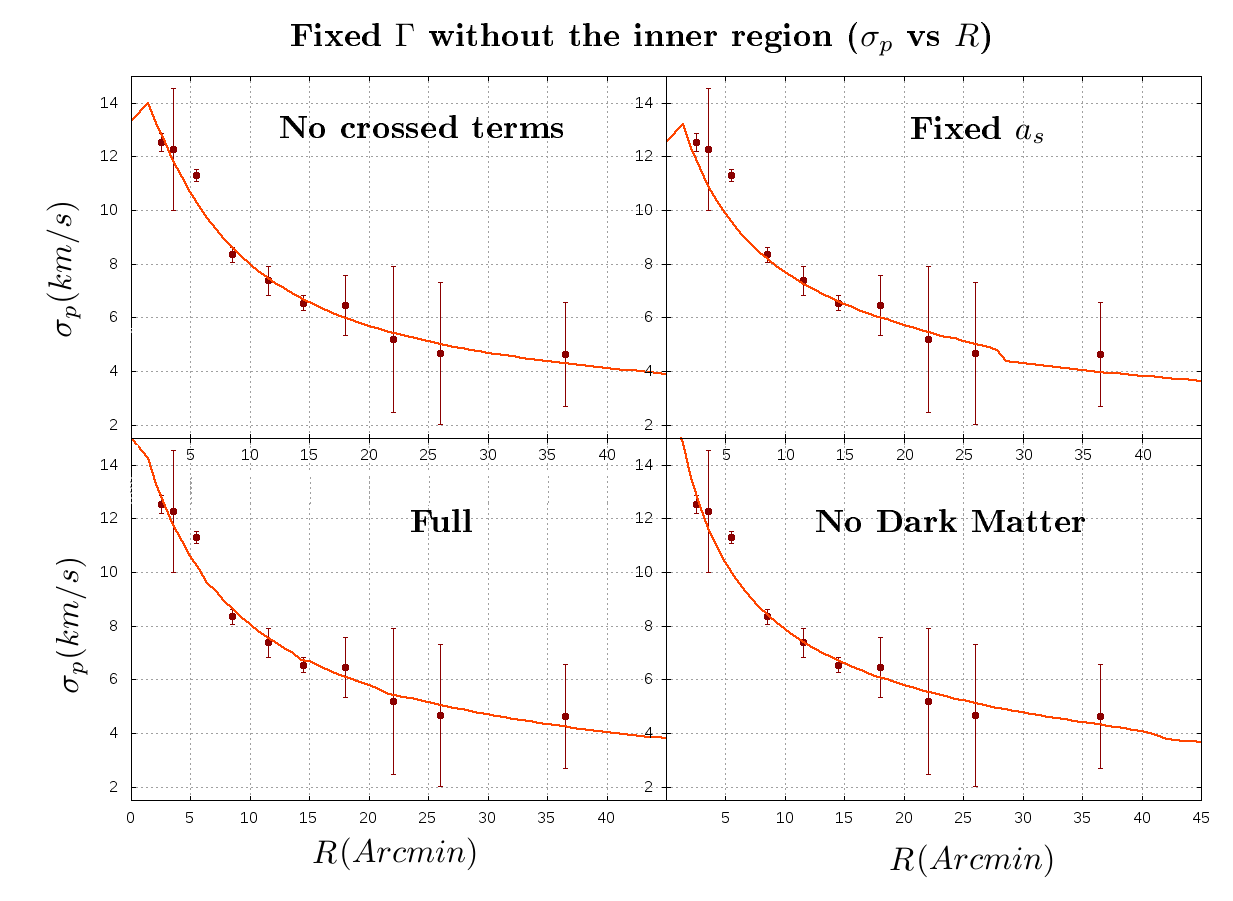
\includegraphics[width=15cm]{images/fix_gamma_refinado_10.png}
\caption[Best fit of our model with a fix mass-to-light ratio for the 10 radial bins]{Best fit to the observational data of the four experiments for our model with a fix mass-to-light ratio with the 10 outer radial bins.}
\end{figure}

\begin{table}[H]
\begin{center}
\begin{tabular}{| c| c| c| c| c| c| c|}
    \hline
    \textbf{Experiment} & $\mathbf{\beta}$ & $\mathbf{a_{dm}} (pc)$ & $\mathbf{a_{s}} (pc)$ & $\mathbf{M_{dm}}$ ($M_{\odot}$) & $\mathbf{M_{s}}$ ($M_{\odot}$) & $\mathbf{\Gamma}$\\ \hline
	No Crossed terms & $0.2$ &	$15.2$ &	$59.8$ &	$1.4 \times 10^{6}$ &	$2.1 \times 10^{6}$ &	$2.5$\\ \hline
	Fix $a_s$ &	$0.801$ &	$3.0$ &	$2.23$ &	$5 \times 10^{5}$ &	$1.0 \times 10 ^{5}$ &	$2.5$\\ \hline
	Full &	$0.9$ &	$16.0$ &	$44.6$ &	$1.62 \times 10^{6}$ &	$1.42 \times 10^{6}$ &	$2.5$\\ \hline
	No Dark Matter &	$0.38$ &	$\thicksim$ & $ a = 2.38$ &	$\thicksim$ & $  M = 2.03 \times 10^{6}$ & 	$2.5$\\
    \hline
  \end{tabular} 
\caption[Optimized parameters for our fix mass-to-light ratio model with the 10 outer radial bins.]{The optimized parameters for each of the experiments for our fix mass-to-light ratio model with the 10 outer radial bins.}
\end{center}
\end{table} 

Now, if we perform the same experiments that we did before but this time we set the constraint of a stellar mass to the mass that we found with Starlight then we would get the following results

\subsection{Fix stellar mass including the inner region of the cluster}

 summarized in figure 4.11 and table 4.5 (for the 12 radial bins)

\begin{figure}[H]
\centering
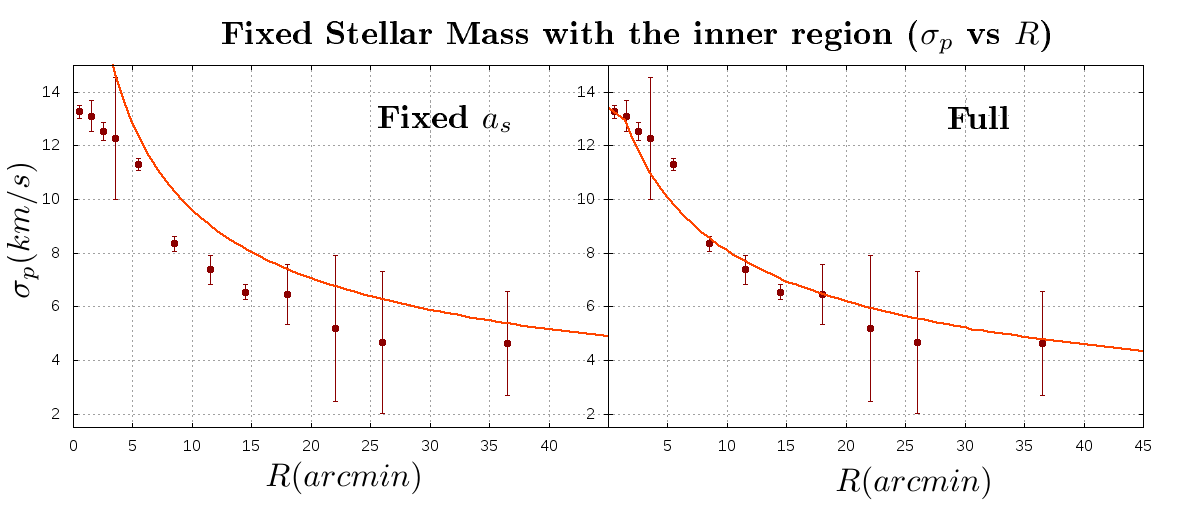
\includegraphics[width=15cm]{images/Starlight_2.png}
\caption[Best fit of our model with the mass found with the Starlight procedures for the 12 radial bins]{Best fit to the observational data of the four experiments for our model with the Starlight procedures for the 12 radial bins. Note that the fitting with a fixed stellar scalength was very bad and didn't give us any valuable results of the parameters.}
\end{figure}

\begin{table}[H]
\begin{center}
\begin{tabular}{| c| c| c| c| c| c| c|}
    \hline
    \textbf{Experiment} & $\mathbf{\beta}$ & $\mathbf{a_{dm}} (pc)$ & $\mathbf{a_{s}} (pc)$ & $\mathbf{M_{dm}}$ ($M_{\odot}$) & $\mathbf{M_{s}}$ ($M_{\odot}$) & $\mathbf{\Gamma}$\\ \hline
	Fix $a_s$ &	$0.88$ &	$56.98$ &	$2.23$ &	$8 \times 10^{4}$ &	$6.61 \times 10 ^{6}$ &	$1.6$\\ \hline
	Full &	$0.96$ &	$7.6$ &	$12.0$ &	$6.88 \times 10^{5}$ &	$6.61 \times 10^{6}$ &	$0.9$\\ \hline
  \end{tabular} 
\caption[Optimized parameters for our model with the mass found with the Starlight procedures for the 12 radial bins.]{The optimized parameters for each of the experiments for our model with the mass found with the Starlight procedures for the 12 radial bins.}
\end{center}
\end{table}

\subsection{Fix stellar mass including for the outer region of the cluster}

the results given in figure 4.12 and table 4.6

\begin{figure}[H]
\centering
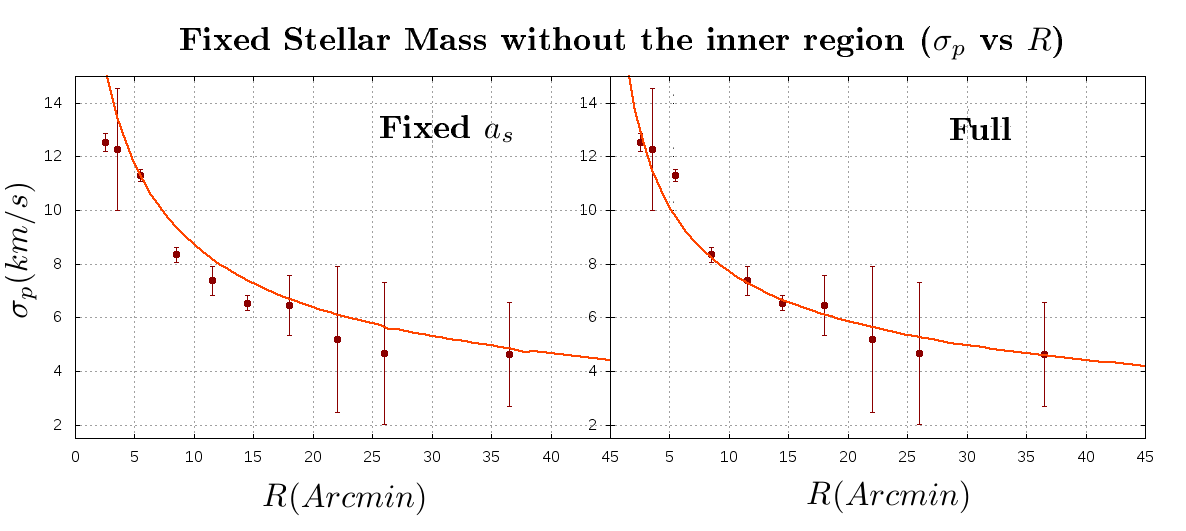
\includegraphics[width=15cm]{images/Starlight_1.png}
\caption[Best fit of our model with the mass found with the Starlight procedures for the 10 outer radial bins]{Best fit to the observational data of the four experiments for our model with the Starlight procedures for the 10 outer radial bins.}
\end{figure}

\begin{table}[H]
\begin{center}
\begin{tabular}{| c| c| c| c| c| c| c|}
    \hline
    \textbf{Experiment} & $\mathbf{\beta}$ & $\mathbf{a_{dm}} (pc)$ & $\mathbf{a_{s}} (pc)$ & $\mathbf{M_{dm}}$ ($M_{\odot}$) & $\mathbf{M_{s}}$ ($M_{\odot}$) & $\mathbf{\Gamma}$\\ \hline
	Fix $a_s$ &	$0.95$ &	$58.0$ &	$2.23$ &	$8 \times 10^{4}$ &	$6.61 \times 10 ^{6}$ &	$2.3$\\ \hline
	Full &	$0.96$ &	$7.36$ &	$50.0$ &	$1.35 \times 10^{6}$ &	$6.61 \times 10^{6}$ &	$1.88$\\ \hline
  \end{tabular} 
\caption[Optimized parameters for our model with the mass found with the Starlight procedures for the 10 outer radial bins.]{The optimized parameters for each of the experiments for our model with the mass found with the Starlight procedures for the 10 outer radial bins.}
\end{center}
\end{table}

\subsection{Starlight's stellar mass final analysis}

As a last experiment, we want to take into account the big error bar in our calculation of the stellar mass found by Starlight, so comparing it with the reported values we decided to use the lowest possible value that an estimated error bar of 25\% would allow us to use. In this case the value of the stellar mass is $M_{s}=4.9 \times 10^{6} M_{\odot}$

For the 12 radial bins the results are shown in figure 4.13 and table 4.7.

\begin{figure}[H]
\centering
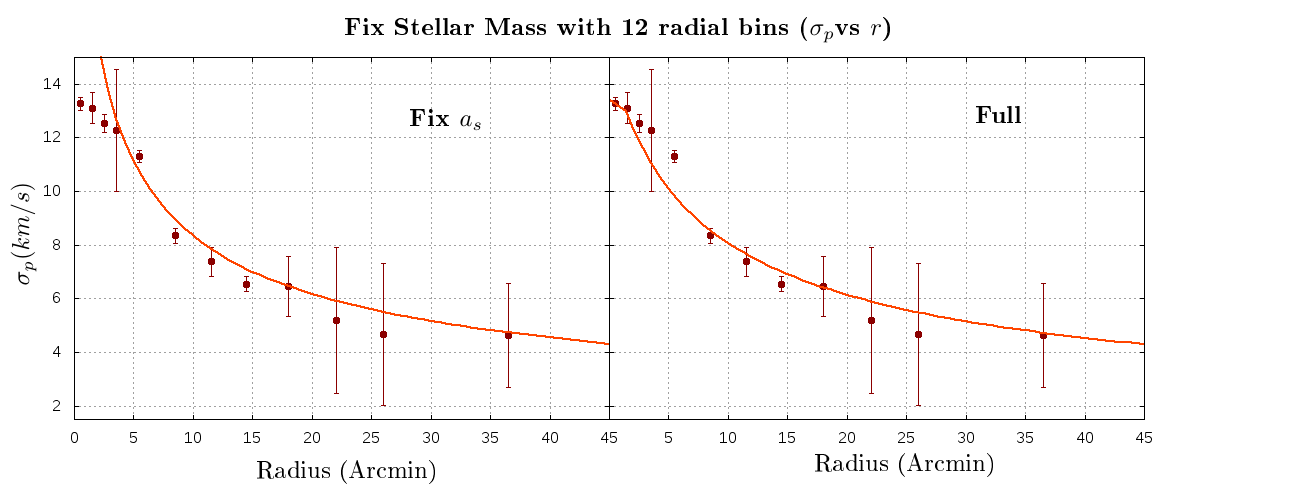
\includegraphics[width=15cm]{images/Starlight_25_12.png}
\caption[Best fits for our model with a mass value based on the Starlight procedures for the 12 radial bins.]{Best fit for each of the experiments for our model with a mass value found with the Starlight procedures for the 12 radial bins.}
\end{figure}

\begin{table}[H]
\begin{center}
\begin{tabular}{| c| c| c| c| c| c| c|}
    \hline
    \textbf{Experiment} & $\mathbf{\beta}$ & $\mathbf{a_{dm}} (pc)$ & $\mathbf{a_{s}} (pc)$ & $\mathbf{M_{dm}}$ ($M_{\odot}$) & $\mathbf{M_{s}}$ ($M_{\odot}$) & $\mathbf{\Gamma}$\\ \hline
	Fix $a_s$ &	$0.88$ &	$56.98$ &	$2.23$ &	$9 \times 10^{4}$ &	$4.9 \times 10 ^{6}$ &	$0.82$\\ \hline
	Full &	$0.98$ &	$13.26$ &	$31.98$ &	$1.98 \times 10^{6}$ &	$4.9 \times 10^{6}$ &	$0.66$\\ \hline
  \end{tabular} 
\caption[Optimized parameters for our model with a mass value based on the Starlight procedures for the 12 radial bins.]{The optimized parameters for each of the experiments for our model with a mass value found with the Starlight procedures for the 12 radial bins.}
\end{center}
\end{table}

And finally, for the 10 outer radial bins, we have the results of the best fits shown in figure 4.14 and table 4.8

\begin{figure}[H]
\centering
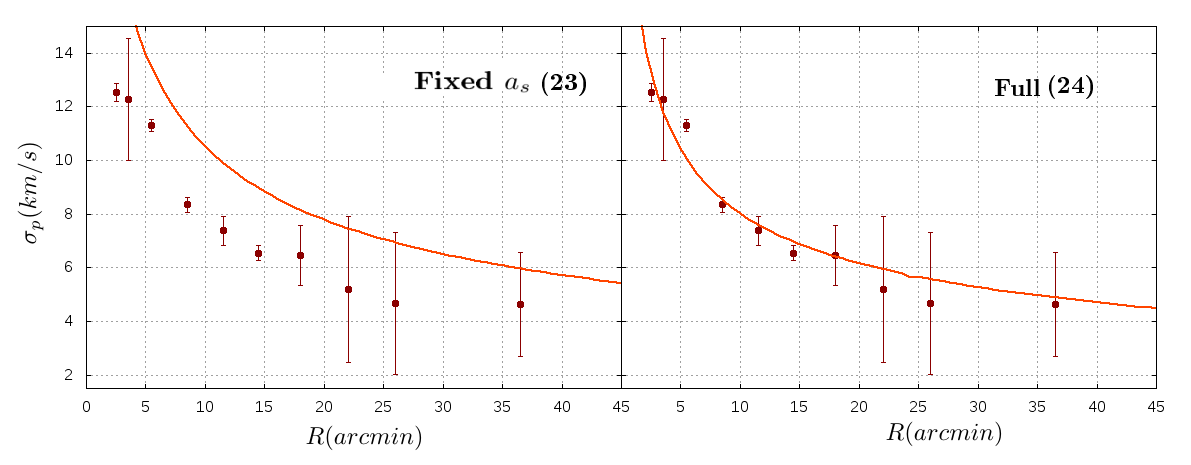
\includegraphics[width=15cm]{images/Starlight_25_10.png}
\caption[Best fits for our model with a mass value based on the Starlight procedures for the 10 outer radial bins.]{Best fit for each of the experiments for our model with a mass value found with the Starlight procedures for the 10 outer radial bins. Note that again, the fitting for the model with the fixed stellar scalength was very bad and didn't give any trustworthy results.}
\end{figure}

\begin{table}[H]
\begin{center}
\begin{tabular}{| c| c| c| c| c| c| c|}
    \hline
    \textbf{Experiment} & $\mathbf{\beta}$ & $\mathbf{a_{dm}} (pc)$ & $\mathbf{a_{s}} (pc)$ & $\mathbf{M_{dm}}$ ($M_{\odot}$) & $\mathbf{M_{s}}$ ($M_{\odot}$) & $\mathbf{\Gamma}$\\ \hline
	Fix $a_s$ &	$0.88$ &	$56.98$ &	$2.23$ &	$9 \times 10^{4}$ &	$4.9 \times 10 ^{6}$ &	$1.1$\\ \hline
	Full &	$0.92$ &	$7.26$ &	$37.98$ &	$1.35 \times 10^{6}$ &	$4.9 \times 10^{6}$ &	$0.72$\\ \hline
  \end{tabular} 
\caption[Optimized parameters for our model with a mass value based on the Starlight procedures for the 10 outer radial bins.]{The optimized parameters for each of the experiments for our model with a mass value found with the Starlight procedures for the 10 outer radial bins.}
\end{center}  
\end{table}

The conclusions of the modelling is discussed in the following chapter.